\documentclass{article}

\usepackage{graphicx}
\usepackage{tikz}
\usepackage{tikzsymbols}
\usetikzlibrary{calc,patterns,shapes.geometric}
\pagestyle{empty}
\usepackage[margin=0pt]{geometry}
\geometry{papersize={14in,12in}}

\def\centerarc[#1](#2)(#3:#4:#5){\draw[#1] ($(#2)+({#5*cos(#3)},{#5*sin(#3)})$) arc (#3:#4:#5);}

\begin{document}
	\begin{figure}
		\centering
		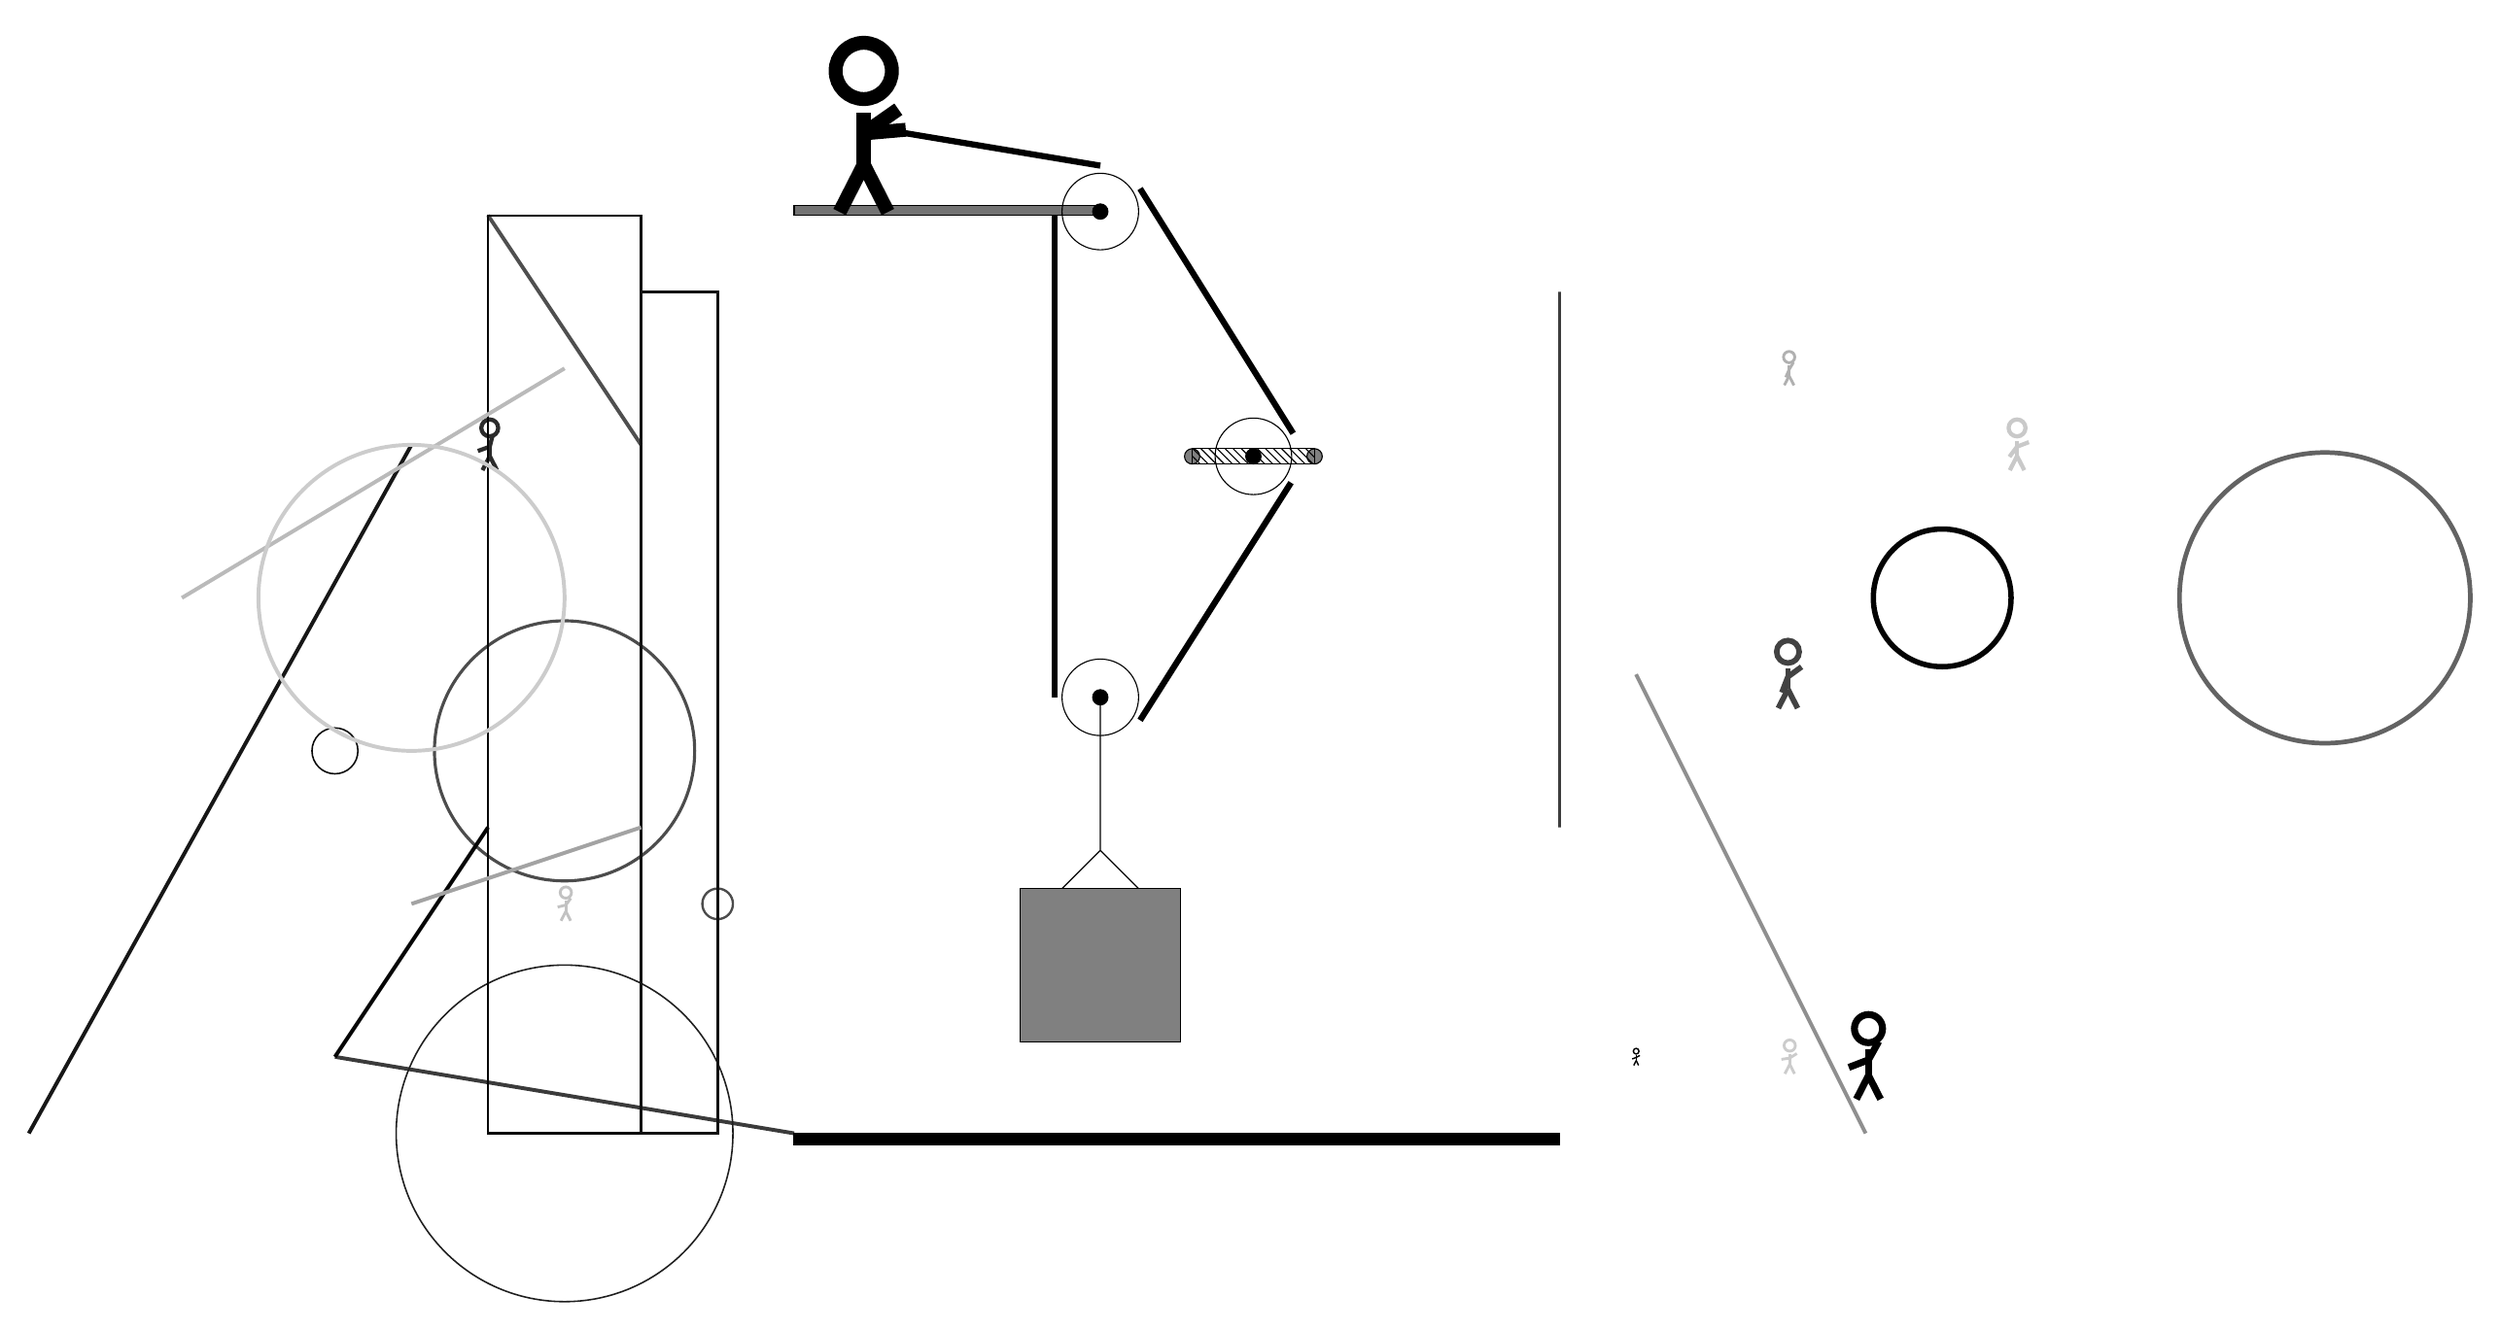
\begin{tikzpicture}
			%%%%% START %%%%%
			
			\draw[fill=black!55] (-2, 9) rectangle (2, 9.125);
			
			\draw (2, 2.7) circle (0.5);
			\draw[fill=black] (2, 2.7) circle (0.1);
			
			\draw (2, 9.05) circle (0.5);
			\draw[fill=black] (2, 9.05) circle (0.1);
			
			\draw[fill=white](4, 5.85) circle (0.5);
			\draw[fill=black] (4, 5.85) circle (0.1);
			\draw[fill=black!50] (3.2, 5.85) circle (0.1);
			\draw[fill=black!50] (4.8, 5.85) circle (0.1);
			\draw[pattern=north west lines, pattern color=black] (3.2, 5.95) rectangle (4.8, 5.75);
			
			\draw (2, 2.7) -- (2, 0.7) -- (1.5, 0.2) -- (2.5, 0.2) -- (2, 0.7);
			\draw[fill=black!50] (0.95, 0.2) rectangle (3.05, -1.8);
			
			\draw[line width=0.8mm] (1.4, 9) -- (1.4, 2.7);
			\centerarc[line width=0.8mm](2, 2.7)(180:330:0.6);
			\draw[line width=0.8mm](2.5196, 2.4) -- (4.4915, 5.5058);
			\centerarc[line width=0.8mm](4, 5.85)(390:325:0.6);
			\draw[line width=0.8mm](4.5196, 6.15) -- (2.5196, 9.35);
			\centerarc[line width=0.8mm](2, 9.05)(30:90:0.6);
			\draw[line width=0.8mm](2, 9.65) -- (-1, 10.15);
			
			\node at (-1, 10.15) {\Strichmaxerl[10][-175][35]};
			
			\draw [line width=0.4mm, color=black!70](-5, 2) circle (1.7);
			
			\draw[line width=0.5mm, color=black!69](-6, 9) -- (-4, 6);
			\node[line width=0.6mm, color=black!74] at (11, 3) {\Strichmaxerl[4][69][36]};
			\draw[line width=0.5mm, color=black!44](9, 3) -- (12, -3);
			\draw[line width=0.3mm, color=black!76] (8, 8) rectangle (8, 1);
			
			\draw[line width=0.5mm, color=black!91](-7, 6) -- (-12, -3);
			\draw[line width=0.5mm, color=black!77](-2, -3) -- (-8, -2);
			
			\draw[line width=0.5mm, color=black!98](-6, 1) -- (-8, -2);
			\draw [line width=0.2mm, color=black!88](-5, -3) circle (2.2);
			
			\draw [line width=0.6mm, color=black!61](18, 4) circle (1.9);
			
			\node[line width=0.7mm, color=black!83] at (-6, 6) {\Strichmaxerl[3][20][76]};
			
			\node[line width=0.7mm, color=black!100] at (12, -2) {\Strichmaxerl[5][21][61]};
			\draw[line width=0.3mm, color=black!97] (-4, 9) rectangle (-6, -3);
			
			\draw [line width=0.3mm, color=black!70](-3, 0) circle (0.2);
			\draw[line width=0.5mm, color=black!27](-5, 7) -- (-10, 4);
			\node[line width=0.6mm, color=black!24] at (-5, 0) {\Strichmaxerl[2][14][54]};
			
			\draw [line width=0.2mm, color=black!96](-8, 2) circle (0.3);
			\node[line width=0.7mm, color=black!20] at (11, -2) {\Strichmaxerl[2][9][32]};
			\node[line width=0.5mm, color=black!31] at (11, 7) {\Strichmaxerl[2][66][59]};
			\node[line width=0.5mm, color=black!99] at (9, -2) {\Strichmaxerl[1][21][28]};
			\draw[line width=0.4mm, color=black!93] (-3, 8) rectangle (-4, -3);
			
			\draw[line width=0.5mm, color=black!36](-7, 0) -- (-4, 1);
			\draw [line width=0.7mm, color=black!99](13, 4) circle (0.9);
			\node[line width=0.6mm, color=black!21] at (14, 6) {\Strichmaxerl[3][53][21]};
			\draw [line width=0.5mm, color=black!20](-7, 4) circle (2.0);
			
			
			\draw[fill=black] (-2, -3) rectangle (8, -3.15);
			
			%%%%% END %%%%%
		\end{tikzpicture}
	\end{figure}	
\end{document}